%\section{Structured Prediction}
\section{Travel Route Recommendation}
% don't need very details of the algorithm
% need problem definition
% copied from nips paper
The travel route recommendation problem involves a set of POIs in a city. 
Given a trajectory query $\mathbf{x} = (s, l)$, comprising a start POI $s$ and trip length $l$, the goal is to suggest one or more sequences of POIs that maximise some notion of utility.

Following~\cite{chen2017SR}, we first cast travel recommendation as a structured prediction problem, which allows us to leverage the well-studied literature of structured SVMs (SSVM)~\cite{joachims2009predicting}. 
%There are two obstacles that prevent us from applying SSVM directly to the sequence recommendation problem; first, there would be multiple ground-truth routes among a set of POIs, second, a naive application of SSVM would generate a loop during prediction time. 
%To incorporate multiple ground-truth routes in the learning phase, we take an idea from the ranking objective which prevents the ground-truth routes from competing with each other~\cite{rendle2009bpr}. 
%To eliminate possible loops in prediction, we adopt the serial list Viterbi algorithm~\cite{seshadri1994list,nill1995list,nilsson2001sequentially}.
%We trained our model on trajectory data extracted from Flickr photos taken in Melbourne~\cite{chen2016learning}.
%
From a visualisation perspective, an advantage of the SSVM is the explicit representation of feature scores in its final decision process. Specifically, we can disassemble the final score of a route into feature scores of each POI and the transition between two adjacent POIs. 
We use hand-crafted POI features such as the category, popularity, and average visit duration of previous tourists. We also crafted transition features such as the distance and neighbourhood of two POIs to maximise the interpretability of the outcome.

\begin{figure}[t!]
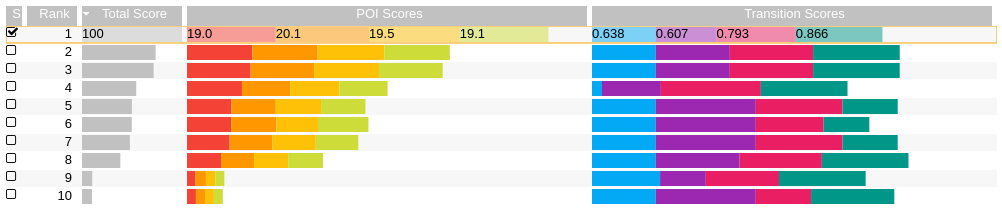
\includegraphics[width=\linewidth]{figure/sample_stack.png} \vspace{-20pt}
\caption{Visualisation of POI and transition scores for top 10 recommended routes. Each bar from left to right represents a relative score of each POI or transition along the route.
The length of stacked bars represents the total score of the suggested route.}
\label{fig:stack} \vspace{-1em}
\end{figure}
